\documentclass[12pt,a4paper]{article}
\usepackage[utf8]{inputenc}
\usepackage[francais]{babel}
\usepackage[T1]{fontenc}
\usepackage{amsmath}
\usepackage{amsfonts}
\usepackage{amssymb}
\usepackage{graphicx}
\usepackage[top=3cm, bottom=3cm, left=3cm, right=3cm]{geometry}

\usepackage{verbatim}

\title{Programmation Logique : Prolog}
\author{Valentin NOEL et Romain Pascual}

\begin{document}
\maketitle

\section{Problème 1 : Traversées de rivière}
Les problèmes des traversée de rivière supposent généralement que l'on doit faire passer des individus d'un côté à l'autre de la rivière en ayant un nombre limité de personnage sur le bateau tout en interdisant à certains personnages de rester ensemble d'un même côté de la rivière.

Ici le problème est le suivant : "Lulu doit faire passer le chou, la chèvre et le loup de l'autre côté de la rivière et il n'a qu'une place sur son bateau. Si la chèvre et le chou sont ensemble sur une rive quand Lulu s'éloigne, la chèvre mange le chou. Et si le loup et la chèvre sont ensemble quand Lulu s'éloigne, le loup mange la chèvre."

On cherche à modéliser le problème en Prolog. La solution est donnée dans le fichier "rivière.pl"

La modélisation est la suivante : on utilise un quadruplet $(Lulu, Chou, Chevre, Loup)$ de booléens tel que chaque variable vaut $0$ si le personnage est du premier côté de la rivière et $1$ s'il est du second. On cherche donc à transformer le tuple $(0,0,0,0,)$ en $(1,1,1,1)$. Pour cela on commence par définir les états interdits (le loup et la chèvre d'un même côté ou encore la chèvre et le chou du même côté). Ensuite on modélise les déplacements possibles : déplacement du chou, de la chèvre, du loup ou de Lulu en interdisant les déplacements qui conduisent à un état interdit.

On cherche ensuite la solution à l'aide d'un parcours en largeur implémenté par des listes.

Le problème est finalement résolu par analogie avec une réflexion sur les graphes où les nœuds représentent les différents états licites et les arcs les déplacements du bateau. La "meilleure" solution est alors obtenue à l'aide d'un parcours en largeur du graphe. Le code du parcours en largeur à été trouvé sur internet et adapté à la situation.

Pour exécuter le code, il suffit d'utiliser la commande \texttt{solution} ou la commande \texttt{solution\_ecrite} dans Prolog après avoir chargé le fichier "rivière.pl". Dans le premier cas, on obtient la liste des situations depuis celle ou tout le monde est sur la première berge jusqu'à celle ou tout le monde est sur la seconde berge. Avec la deuxième commande, on obtient la liste écrite des déplacements de Lulu, comme le montre la sortie ci-dessous :

\begin{center}
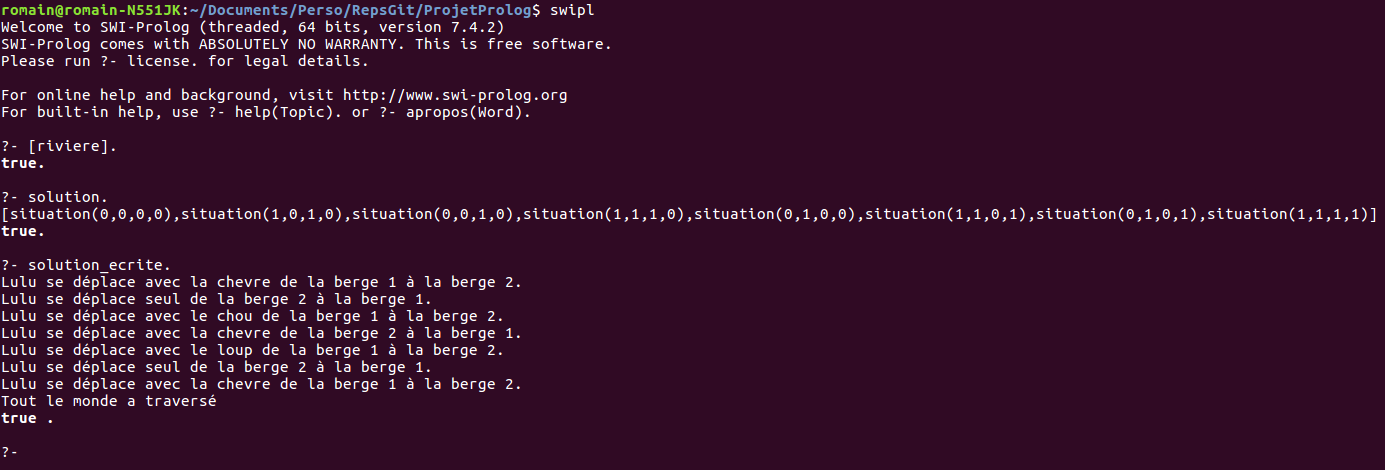
\includegraphics[width = 425pt]{SolutionRiviere.png}
\end{center}



\section{Problème 2 : Le compte est bon}
"Le compte est bon est un jeu (télévisé) qui consiste à trouver une combinaison arithmétique de nombres afin d'obtenir un certain total."

\end{document}